%!TEX root=./paper.tex
\subsection{Results}

\begin{figure*}[]
  \centering
  \begin{subfigure}[b]{0.9\textwidth}
      \centering
      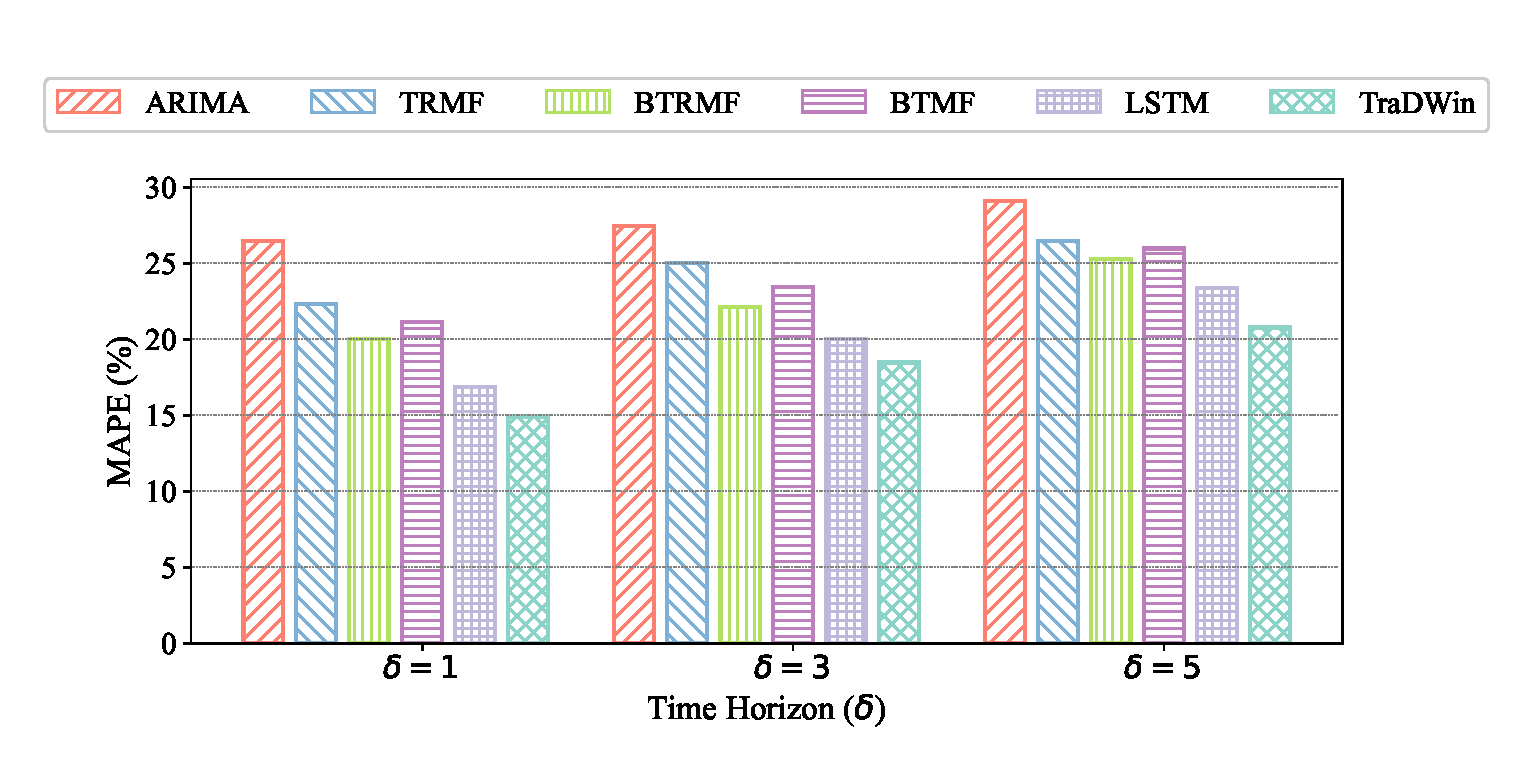
\includegraphics[width=\textwidth]{mape_pred.eps}
      \caption{MAPE on prediction task for different deltas}
      \label{fig:mape_pred}
  \end{subfigure}
  
  \begin{subfigure}[b]{0.9\textwidth}
      \centering
      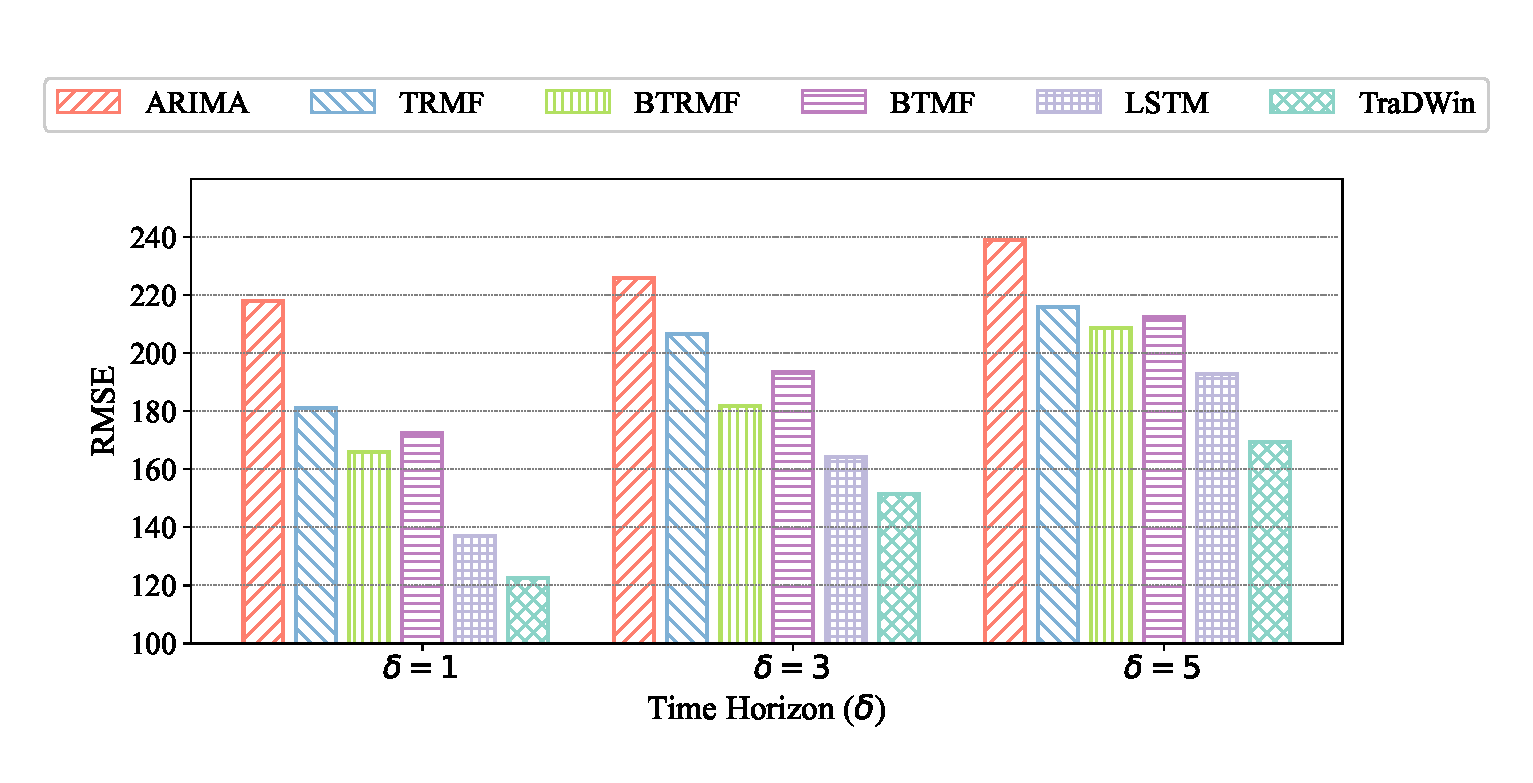
\includegraphics[width=\textwidth]{rmse_pred.eps}
      \caption{RMSE on prediction task for different deltas}
      \label{fig:rmse_pred}
  \end{subfigure}
  
  \caption{Performance metrics on prediction task for different deltas (timesteps to predict ahead)}
  \label{fig:pred_metrics}
\end{figure*}

We evaluate the performance of our model on the following tasks, which cover various scenarios related to traffic modelling, along with comparing to other popular models in the domain.

\subsection*{(i) Prediction}

For the prediction task, we test the models for predicting traffic volumes at the next timestep (\(\delta = 1\)), at the third timestep (\(\delta = 3\)), and at the fifth timestep in the future (\(\delta = 5\)). This scenario requires a mask consisting of all the \(T_{n+1}\) values missing, i.e., 0, for the next timestep prediction. We similarly prepare a mask for other time horizons, treating prediction as a strict MNAR (Missing Not At Random) subcategory of imputation.

The MAPE and RMSE plots of prediction tasks across different horizons are shown in Fig. \ref{fig:mape_pred} and Fig. \ref{fig:rmse_pred}, respectively. We observe that generally, as the time horizon \(\delta\) increases, both metrics worsen, with MAPE falling 5-10\% from \(\delta=1\) to \(\delta=3\). This indicates a stronger short-term accuracy but some challenges with long-term prediction across all models. This trend is common in time-series forecasting, where predictive accuracy decreases as the prediction horizon extends. The primary reasons for this decline include the increasing uncertainty and the influence of unpredictable external factors, such as accidents or weather changes.

\begin{figure*}[]
  \centering
  \begin{subfigure}{0.5\textwidth}
    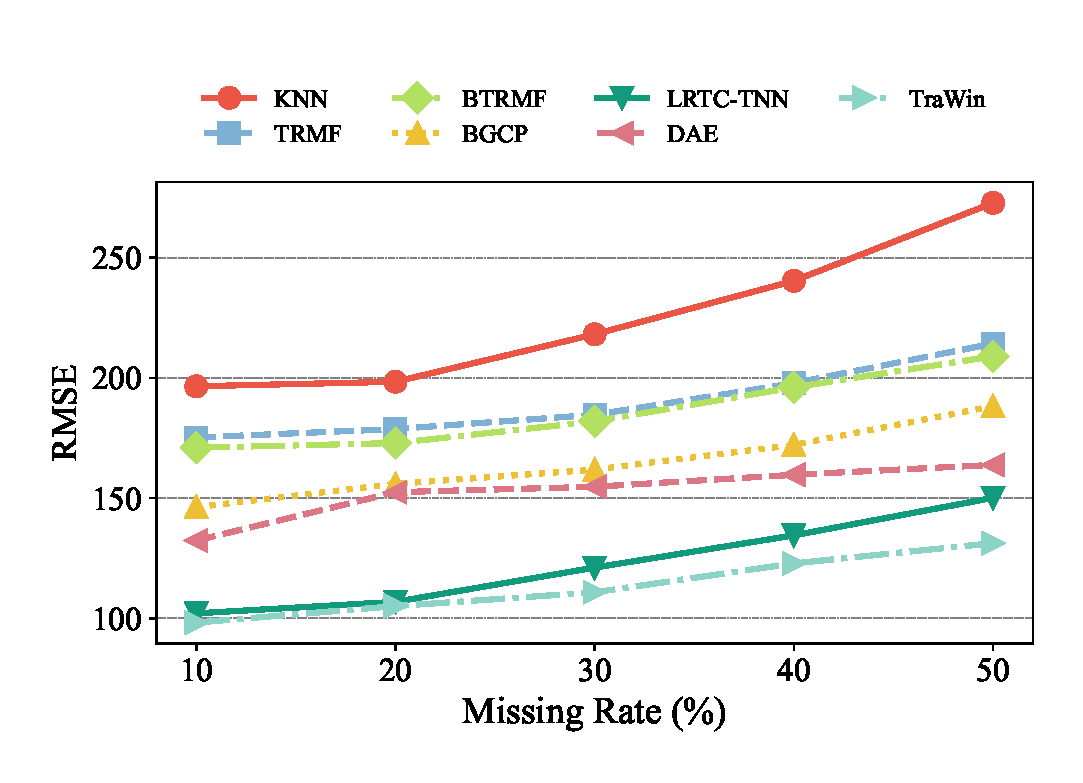
\includegraphics[width=\linewidth]{rmse_imput.eps}
    \caption{RMSE of different models on imputation task}
    \label{fig:mape_imput}
  \end{subfigure}%
  \begin{subfigure}{0.5\textwidth}
    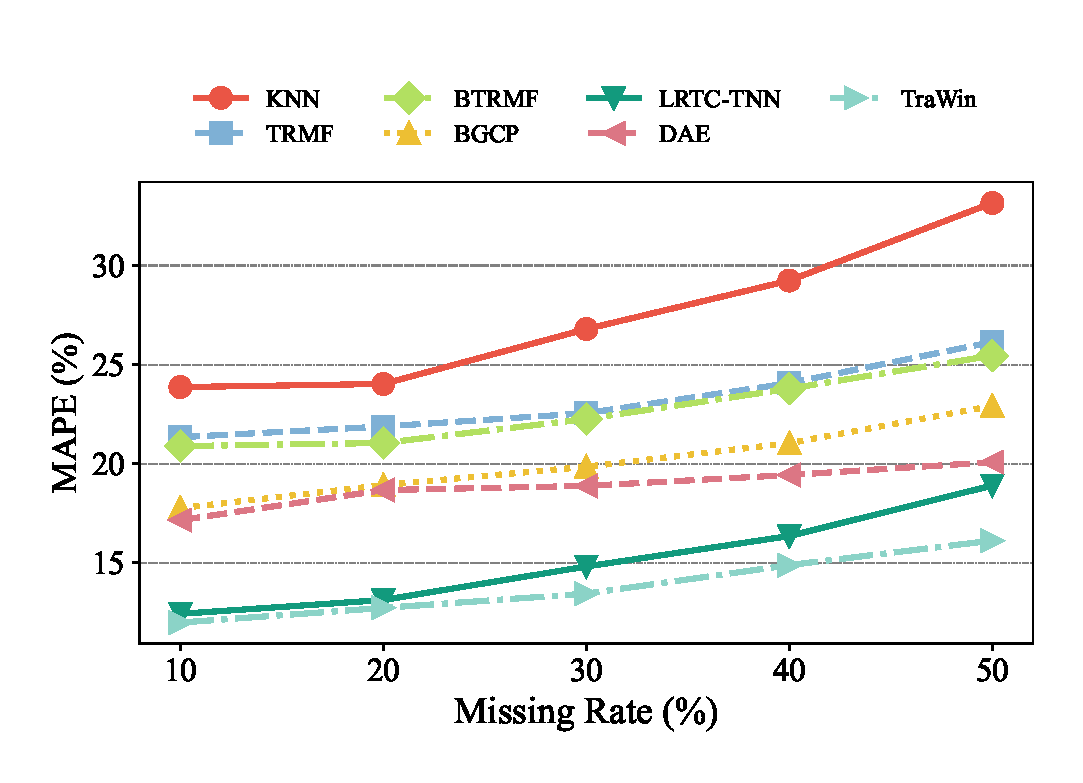
\includegraphics[width=\linewidth]{mape_imput.eps}
    \caption{MAPE of different models on imputation task}
    \label{fig:rmse_imput}
  \end{subfigure}
  \caption{Imputation comparison for different missing rates}
  \label{fig:imput}
  \end{figure*}

ARIMA performs the worst, which is expected as it is the simplest of the mathematical models among the baselines we consider. Other matrix factorization and Bayesian models like TRMF, BTRMF, and BTMF perform better but, being strictly mathematical models, they (i) fail to capture the intricate traffic dynamics that a deep learning model can and (ii) use only the time-series traffic data and not the graph topology and external factors, such as weather, that our model considers. LSTMs perform close but slightly worse (by 2-3\%), likely due to the lack of knowledge of graph topology that our model incorporates through Node2Vec.

Overall, our \name\ model performs significantly better than most models, scoring roughly 3 to 7 percentage points better than the baselines.

\subsection*{(ii) Imputation}

For the imputation task task, we consider the MCAR (Missing Completely At Random) distribution and compare the models at five missing rates of $10\%$, $20\%$, $30\%$, $40\%$, and $50\%$. The performance of different models, measured using MAPE and RMSE, is shown in Fig. \ref{fig:imput}. Conventional methods like KNN perform poorly compared to more specialized approaches, as expected, since KNN is insufficient to capture intricate traffic dynamics. Matrix factorization and Bayesian methods, such as TRMF, BTRMF, and BGCP, work slightly better, with deep learning methods like DAE performing ahead. However, since they deal only with traffic data time series without topology information, their performance is 8-13\% worse than our model. Tensor completion-based models like LRTC-TNN are close to our \name\ for low missing rates but do not scale as well with increasing missing rates. This could be because too much data is lost for reliable tensor completion, which a deep learning model can handle due to its ability to learn complex data relationships and incorporate graph topology and other external factors. It is also worth noting that LRTC-TNN, an MCAR imputer, is not applicable to task (iii) and is not generalized enough for our use case. For all models, the accuracy of imputations decreases with higher missing rates due to the reduced amount of contextual information available, a common challenge in data imputation. Overall, our \name\ scales well with more missing data and performs significantly (5-7\%) better than the compared baselines.

We observe that \name\ performs better on task (ii) than on task (i) by around 4\%. One primary reason for this could be that GAIN, originally designed for MCAR imputation, does not generalize well to MNAR imputation scenarios. Another possible reason could be the subgraph-based computation method we use, where nodes at the corners of the subgraph lack adequate spatial and temporal information about their neighbors. Overall, our model performs reasonably and delivers comparable results as a generalized model on both tasks.

\subsection*{\textit(iii) Re-assignment}
For the re-assignment task, which is a new task addressed in our paper and not commonly seen in contemporary literature, we train the model for MNAR imputation scenarios with the central node cluster missing. This training effectively teaches the model to assign traffic to node clusters based on neighbor node information. To elaborate, for a modified edge, nodes around the edge, based on a distance threshold, are masked (i.e., marked missing). The training input includes features for the neighbors of the cluster (nodes not masked out), graph embeddings for the masked nodes (not the traffic volume as that is marked missing), and the total volume of traffic for the masked-out nodes. The task is to assign traffic volumes to the masked-out nodes and compare them against the original values. The model learns "traffic assignment" since real-world labeled data for traffic state before and after modification of edges is unavailable. Based on this training task, we achieve a MAPE of $13.47\%$ and RMSE of $109.90$. The other baselines considered for prediction and imputation are not applicable without changes to their model architecture, so there is no comparison with contemporary models.

The de-facto way to solve this problem, as observed in our literature review, has been through simulations like SUMO\cite{sumo} and Vissim\cite{vissim}. Using SUMO, we also compare and test our model on the TAPASCologne scenario. We train using the same approach as for the Dublin SCATS dataset but test against the simulation results after modifying the said edge. This is not possible for the Dublin dataset since detailed origin-destination pair data is unavailable. The results of our model on this task are shown in Table \ref{reassign_table}. We observe that the model achieves a MAPE of $13.47\%$ on the Dublin SCATS dataset and $15.06\%$ on the TAPASCologne scenario, demonstrating the model's reasonable accuracy in solving the traffic assignment problem on node clusters. Furthermore, we evaluate how our model's performance scales with the number of modifications, i.e., how much we can alter the original graph while keeping the model viable for re-assignment. Fig. \ref{fig:edge_modif} shows a comparison of MAPE and RMSE with the number of edges modified. Performance declines steadily from $13.47\%$ at one change to $31.91\%$ at five changes, indicating that more graph alterations lead to a significant performance drop, especially after three modifications. A possible reason for this could be the mass masking strategy used to train the model for task (iii), where masking too many neighboring nodes leads to a large loss of contextual information that graph representation knowledge cannot fully compensate.


\begin{figure}[t]
  \centering
  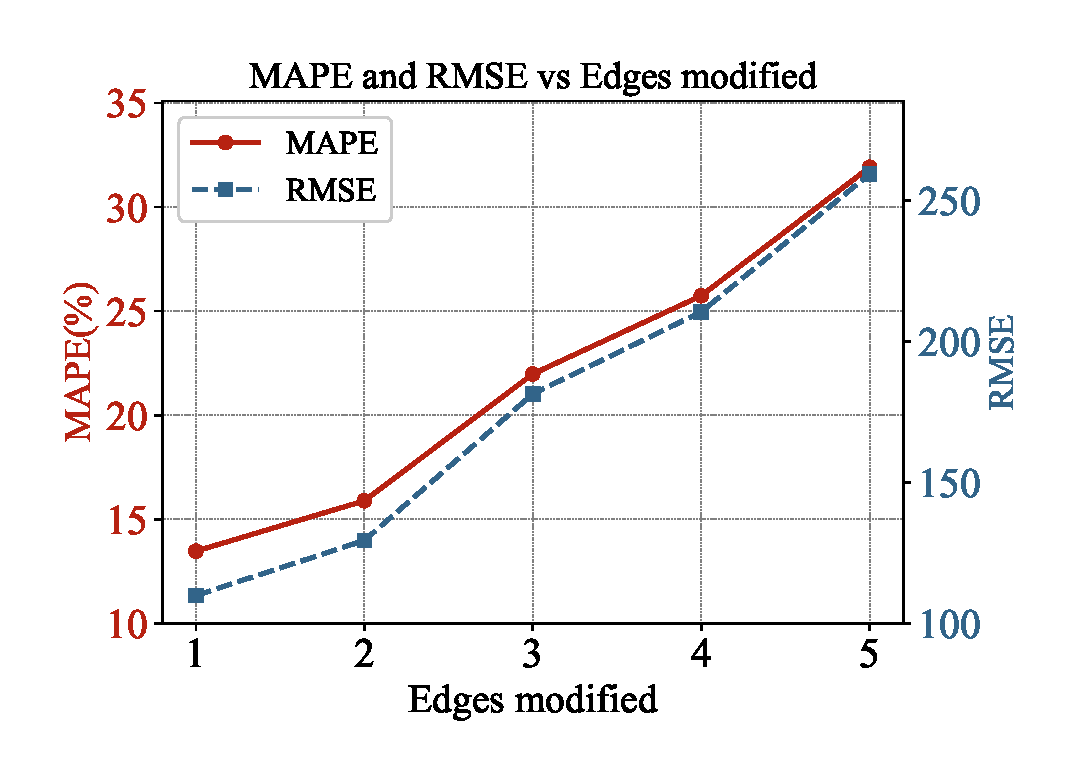
\includegraphics[width=\linewidth]{modif.eps}
  \caption{MAPE and RMSE on re-assignment task vs number of edges modified}
  \label{fig:edge_modif}
\end{figure}

\begin{table}[]
\centering
\caption{Performance on re-assignment task (1 edge change) for different datasets}
\label{reassign_table}
\begin{tabular}{lcc}
\toprule
Dataset & MAPE (\%) & RMSE \\
\midrule
Dublin SCATS & 13.47 & 109.90 \\
TAPASCologne & 15.06 & 23.34 \\
\bottomrule
\end{tabular}
\end{table}